\documentclass[../main-sheet.tex]{subfiles}
\usepackage{../style}
\graphicspath{ {../img/} }
\backgroundsetup{contents={}}
\begin{document}
\section{Problems}
\begin{prob}
    Employ the method of isoclines to sketch several approximate integral curves of the following differential equations.
    \begin{enumerate}[label=(\alph*)]
        \item \(\ddx{y}=x^2+y^2\)
        \item \(\ddx{y}=y^3-x^2\)
        \item \(\ddx{y}=\frac{y}{x^2}\)
    \end{enumerate}
\end{prob}
\begin{soln}[a]
    \begin{equation}
        \ddx{y}=x^2+y^2\label{eq:iso1a.1}
    \end{equation}
    and the isocline of \eqref{eq:iso1a.1} is given by 
    \begin{align}
        &\ddx{y}=c\notag\\
        \Rightarrow\,&x^2+y^2=c\label{eq:iso1a.2}
    \end{align}
    Where \(c\) is the slope of the line element of the curves obtained for different values of \(c\).\\
    For different values of parameter \(c\) \eqref{eq:iso1a.2} represent a family of circle.\\
    We construct the curve \eqref{eq:iso1a.2} for \(c=0,\,0.5,\,0.75,\,1,\,1.5,\,2,\,3\) etc.\\
    On each of these circles we then construct a number of line elements having the approximate inclinations \(\tan^{-1}c\).
    \begin{align*}
        \text{When } & c=0,  & \text{ then } & x^2+y^2=0,   &&\theta=\tan^{-1}c=0^{\circ}\\
        \text{When } & c=0.5,  & \text{ then } & x^2+y^2=0.5, &&\theta=\tan^{-1}c=26.56^{\circ}\\
        \text{When } & c=0.75, & \text{ then } & x^2+y^2=0.75, &&\theta=\tan^{-1}c=36.86^{\circ}\\
        \text{When } & c=1,  & \text{ then } & x^2+y^2=1, &&\theta=\tan^{-1}c=45^{\circ}\\
        \text{When } & c=1.5, & \text{ then } & x^2+y^2=1.5, &&\theta=\tan^{-1}c=56.3^{\circ}\\
        \text{When } & c=2, & \text{ then } & x^2+y^2=2, &&\theta=\tan^{-1}c=63.43^{\circ}\\
        \text{When } & c=3, & \text{ then } & x^2+y^2=3, &&\theta=\tan^{-1}c=71.56^{\circ}
    \end{align*}
    \begin{figure}[H]
        \centering
        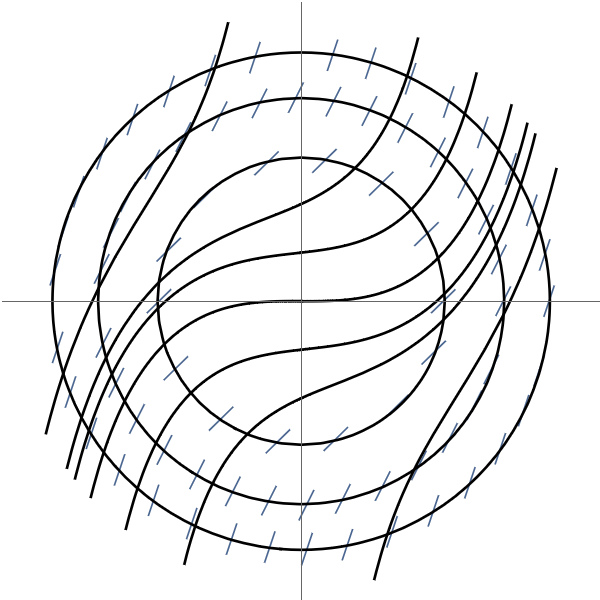
\includegraphics{pr1.png}
        % \import{../tikz/}{iso-1.tikz}
    \end{figure}
    Finally we draw several smooth curves. These smooth curves represent the approximate integral curves of \eqref{eq:iso1a.1}.
\end{soln}
\begin{soln}[b]
    \begin{equation}
        \ddx{y}=y^3-x^2\label{eq:iso1b.1}
    \end{equation}
    and the isocline of \eqref{eq:iso1b.1} is given by 
    \begin{align}
        &\ddx{y}=c\notag\\
        \Rightarrow\,&y^3-x^2=c\label{eq:iso1b.2}
    \end{align}
    Where \(c\) is the slope of the line element of the curves obtained for different values of \(c\).\\
    For different values of parameter \(c\) \eqref{eq:iso1b.2} represent a family of curves.\\
    We construct the curve \eqref{eq:iso1b.2} for \(c=0,\,\pm 1,\,\pm23\) etc.\\
    On each of these circles we then construct a number of line elements having the approximate inclinations \(\tan^{-1}c\).
    % \begin{align*}
    %     \text{When } & c=0,  & \text{ then } & x^2+y^2=0,   &&\theta=\tan^{0}c=0^{\circ}\\
    %     \text{When } & c=0.5,  & \text{ then } & x^2+y^2=0.5, &&\theta=\tan^{0.5}c=26.56^{\circ}\\
    %     \text{When } & c=0.75, & \text{ then } & x^2+y^2=0.75, &&\theta=\tan^{0.75}c=36.86^{\circ}\\
    %     \text{When } & c=1,  & \text{ then } & x^2+y^2=1, &&\theta=\tan^{1}c=45^{\circ}\\
    %     \text{When } & c=1.5, & \text{ then } & x^2+y^2=1.5, &&\theta=\tan^{1.5}c=56.3^{\circ}\\
    %     \text{When } & c=2, & \text{ then } & x^2+y^2=2, &&\theta=\tan^{2}c=63.43^{\circ}\\
    %     \text{When } & c=3, & \text{ then } & x^2+y^2=3, &&\theta=\tan^{3}c=71.56^{\circ}
    % \end{align*}
    When \(c=0\), then \(y^3=x^2\), \(\theta=\tan^{-1}c=0^{\circ}\)\\
    \(c=0\) \begin{tabular}{|c|c|c|c|c|c|c|}
        \hline
        \(x\) & 0& \(\pm 0.35\) & \(\pm 1\) & \(\pm 1.84\) & \(2.83\) & \(\pm 3.95\)\\\hline
        \(y\) & 0& 0.5 & 1 & 1.5 & 2 & 2.5\\\hline
    \end{tabular}\\
    When \(c=1\), then \(y^3=x^2+1\), \(\theta=\tan^{-1}c=45^{\circ}\)\\
    \(c=1\) \begin{tabular}{|c|c|c|c|c|}
        \hline
        \(x\) & 0& \(\pm 1.54\) & \(\pm 2.65\) & \(\pm 3.82\)\\\hline
        \(y\) & 1& 1.5 & 2 & 2.5 \\\hline
    \end{tabular}\\
    When \(c=-1\), then \(y^3=x^2-1\), \(\theta=\tan^{-1}c=-45^{\circ}\)\\
    \(c=-1\) \begin{tabular}{|c|c|c|c|c|c|c|c|}
        \hline
        \(x\) & 0& \(\pm 0.94\) & \(\pm 1\) & \(\pm 1.06\)& \(\pm 1.4\)& \(\pm 2.03\)& \(\pm 3\)\\\hline
        \(y\) & -1& -0.5 & 0 & 0.5&1&1.5&2 \\\hline
    \end{tabular}\\
    When \(c=2\), then \(y^3=x^2+2\), \(\theta=\tan^{-1}c=63.43^{\circ}\)\\
    \(c=2\) \begin{tabular}{|c|c|c|c|c|c|c|c|c|c|}
        \hline
        \(x\) & 0& \(\pm 0.5\) & \(\pm 1\) & \(\pm 1.5\)& \(\pm 2\)& \(\pm 2.44\)& \(\pm 3\)&\(\pm 3.69\)&\(\pm 4\)\\\hline
        \(y\) & 1.25& 1.31 & 1.44 & 1.61&1.81&2&2.22&2.5&2.62 \\\hline
    \end{tabular}\\
    When \(c=-2\), then \(y^3=x^2-2\), \(\theta=\tan^{-1}c=-63.43^{\circ}\)\\
    \(c=-2\) \begin{tabular}{|c|c|c|c|c|c|c|c|c|}
        \hline
        \(x\) & 0& \(\pm 1\) & \(\pm 1.5\) & \(\pm 2\)& \(\pm 2.3\)& \(\pm 3.16\)& \(\pm 3.65\)&\(\pm 4\)\\\hline
        \(y\) & -1.25& -1 & 0.62 & 1.25&1.5&2&2.25&2.41 \\\hline
    \end{tabular}\\
    %     \text{When } & c=0.5,  & \text{ then } & x^2+y^2=0.5, &&\theta=\tan^{0.5}c=26.56^{\circ}\\
    %     \text{When } & c=0.75, & \text{ then } & x^2+y^2=0.75, &&\theta=\tan^{0.75}c=36.86^{\circ}\\
    %     \text{When } & c=1,  & \text{ then } & x^2+y^2=1, &&\theta=\tan^{1}c=45^{\circ}\\
    %     \text{When } & c=1.5, & \text{ then } & x^2+y^2=1.5, &&\theta=\tan^{1.5}c=56.3^{\circ}\\
    %     \text{When } & c=2, & \text{ then } & x^2+y^2=2, &&\theta=\tan^{2}c=63.43^{\circ}\\
    %     \text{When } & c=3, & \text{ then } & x^2+y^2=3, &&\theta=\tan^{3}c=71.56^{\circ}
    % \end{align*}
    \begin{figure}[H]
        \centering
        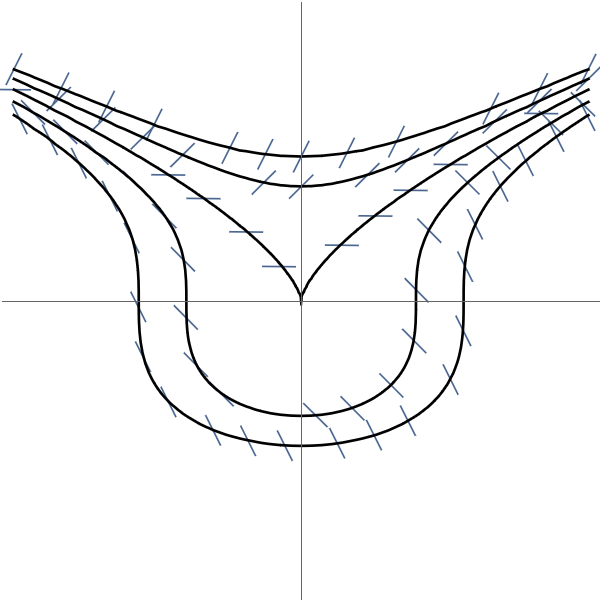
\includegraphics{pr1b.png}
        % \import{../tikz/}{iso-1.tikz}
    \end{figure}
    Finally we draw several smooth curves. These smooth curves represent the approximate integral curves of \eqref{eq:iso1b.1}.
\end{soln}
\begin{soln}[c]
    \begin{equation}
        \ddx{y}=\frac{y}{x^2}\label{eq:iso1c.1}
    \end{equation}
    and the isocline of \eqref{eq:iso1c.1} is given by 
    \begin{align}
        &\ddx{y}=c\notag\\
        \Rightarrow\,&\frac{y}{x^2}=c\notag\\
        \Rightarrow\,&{y}=c{x^2}\label{eq:iso1c.2}
    \end{align}
    Where \(c\) is the slope of the line element of the curves obtained for different values of \(c\).\\
    For different values of parameter \(c\) \eqref{eq:iso1b.2} represent a family of parabola.\\
    We construct the curve \eqref{eq:iso1b.2} for \(c=0,\,\pm 1,\,\pm 2\) etc.\\
    On each of these circles we then construct a number of line elements having the approximate inclinations \(\tan^{-1}c\).
    \begin{align*}
        \text{When } & c=0,  & \text{ then } & y=0,   &&\theta=0^{\circ}\\
        \text{When } & c=1,  & \text{ then } & y=x^2, &&\theta=45^{\circ}\\
        \text{When } & c=-1, & \text{ then } & y=x^2, &&\theta=-45^{\circ}\\
        \text{When } & c=2,  & \text{ then } & y=2x^2, &&\theta=63.43^{\circ}\\
        \text{When } & c=-2, & \text{ then } & y=-2x^2, &&\theta=-63.43^{\circ}\\
        \text{When } & c=\infty, & \text{ then } & x=0, &&\theta=90^{\circ}
    \end{align*}
    \begin{figure}[H]
        \centering
        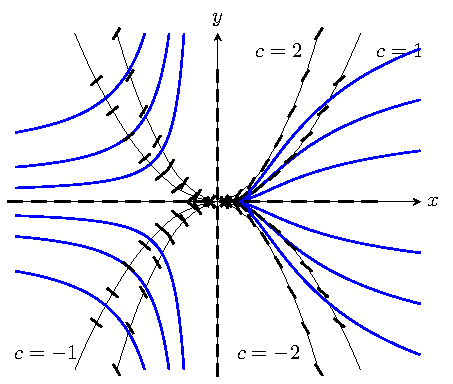
\includegraphics[scale=2]{pr3.pdf}
        % \import{../tikz/}{pr3.tikz}
    \end{figure}
    Finally we draw several smooth curves. These smooth curves represent the approximate integral curves of \eqref{eq:iso1c.1}.
\end{soln}
\begin{prob}
    Examine the nature and stability of the critical points of the following autonomous system and sketch the phase portrait of each cases.
    \begin{enumerate}[label=(\alph*)]
        \item \(\begin{aligned}[t]
            \ddt{x}&=x+x^2-3xy\\
            \ddt{y}&=-2x+y+3y^2
        \end{aligned}\)
        \item \(\begin{aligned}[t]
            \ddt{x}&=x(4-2x-4y)\\
            \ddt{y}&=y(x-1)
        \end{aligned}\)
        \item \(\begin{aligned}[t]
            \ddt{x}&=y-x^2\\
            \ddt{y}&=8x-y^2
        \end{aligned}\)
    \end{enumerate}
\end{prob}
\begin{soln}[a]
    We have
    \begin{equation}
        \begin{rcases}
            \displaystyle\dot{x}=x+x^2-3xy\quad\\
            \displaystyle\dot{y}=-2x+y+3y^2
        \end{rcases}
        \label{eq:p2a.1}
    \end{equation}
    The critical point of the system \eqref{eq:p2a.1} are given by \(\dot{x}=0\) and \(\dot{y}=0\). i.e.,
    \begin{align}
        x+x^2-3xy&=0\label{eq:p2a.2}\\
        -2x+y+3y^2&=0\label{eq:p2a.3}
    \end{align}
    From \eqref{eq:p2a.2} we get,
    \begin{align*}
        x&=0, \qquad 1+x-3y=0\\
        &\qquad\quad\Rightarrow\,x=3y-1
    \end{align*}
    Putting \(x=0\) in \eqref{eq:p2a.3} we get,
    \begin{align*}
        &y+3y^2=0\\
        \Rightarrow\;&y(1+3y)=0\\
        \Rightarrow\;&y=0,\quad y=-\frac{1}{3}
    \end{align*}
    Again put \(x=3y-1\) in \eqref{eq:p2a.3} we get,
    \begin{align*}
        &-6y+2+y+3y^2=0\\
        \Rightarrow\;&3y^2-5y+2=0\\
        \Rightarrow\;&y=1,\quad y=\frac{2}{3}
    \end{align*}
    Hence the critical points are \((0,0)\), \((0,-\frac{1}{3})\), \((2,1)\), \((1,\frac{2}{3})\).\\
    
    \emph{(I) Investigation for critical point \((0,0)\):}\\
    The corresponding linearized system of \eqref{eq:p2a.1} is 
    \begin{equation}
        \begin{rcases}
            \dot{x}=x\\
            \dot{y}=-2x+y\quad
        \end{rcases}
        \label{eq:p2a.4}
    \end{equation}
    Here we observe that
    \begin{enumerate}[label=(\roman*)]
        \item \(\begin{vmatrix}
            a&b\\
            c&d
        \end{vmatrix}=\begin{vmatrix}
            1&0\\
            -2&1
        \end{vmatrix}\neq 0\)
        \item \(\displaystyle\lim_{\substack{x\to 0 \\ y\to 0}} \frac{P(x,y)}{\sqrt{x^2+y^2}}=\lim_{\substack{x\to 0 \\ y\to 0}} \frac{Q(x,y)}{\sqrt{x^2+y^2}}=0\)\\ 
        
        Where \(P(x,y)=x^2-3xy\); \(Q(x,y)=3y^2\)
    \end{enumerate}
    Hence the behavior of the paths of the system \eqref{eq:p2a.1} near \((0,0)\) would be similar to that of the paths of the related linearized system \eqref{eq:p2a.4}.\\
    The characteristic equation of \eqref{eq:p2a.4} is
    \begin{align*}
        &\lambda^2-(1+1)\lambda+1-0=0\\
        \Rightarrow\;&\lambda^2-2\lambda+1=0\\
        \Rightarrow\;&(\lambda-1)^2=0\\
        \Rightarrow\;&\lambda=1,\;\;1
    \end{align*}
    The characteristic roots are real, equal and positive. Thus, the critical points \((0,0)\) is unstable node.\\
    
    
    \emph{(II) Investigation for critical point \((0,-\frac{1}{3})\):}\\
    For the critical point \((0,-\frac{1}{3})\) we make the transformation \(x=\xi\), \(y=\eta-\frac{1}{3}\). So that \(\dot{x}=\dot{\xi}\), \(\dot{y}=\dot{\eta}\). Which transforms the critical point \(x=0\), \(y=-\frac{1}{3}\) to \(\xi=0\), \(\eta=0\) in the \(\xi\eta\) plane.\\
    With this transformation, we get from \eqref{eq:p2a.1}
    \begin{align}
        &\dot{\xi}=\xi+\xi^2-3\xi\left(\eta-\frac{1}{3}\right)\notag\\
        &\dot{\eta}=-2\xi+\eta-\frac{1}{3}+3\left(\eta-\frac{1}{3}\right)^2\notag\\
        \Rightarrow\;\;&\begin{aligned}
            \begin{rcases}
                \dot{\xi}=2\xi+\xi^2-3\xi\eta\quad\\
                \dot{\eta}=-2\xi-\eta+3\eta^2
            \end{rcases}
        \end{aligned}\label{eq:p2a.5}
    \end{align}
    The corresponding linearized system of \eqref{eq:p2a.5} is 
    \begin{equation}
        \begin{rcases}
            \dot{\xi}=2\xi\\
            \dot{\eta}=-2\xi-\eta\quad
        \end{rcases}
        \label{eq:p2a.6}
    \end{equation}
    Here we observe that
    \begin{enumerate}[label=(\roman*)]
        \item \(\begin{vmatrix}
            a&b\\
            c&d
        \end{vmatrix}=\begin{vmatrix}
            2&0\\
            -2&-1
        \end{vmatrix}\neq 0\)
        \item \(\displaystyle\lim_{\substack{\xi\to 0 \\ \eta\to 0}} \frac{P_1(\xi,\eta)}{\sqrt{\xi^2+\eta^2}}=\lim_{\substack{\xi\to 0 \\ \eta\to 0}} \frac{Q_1(\xi,\eta)}{\sqrt{\xi^2+\eta^2}}=0\)\\ 
        
        Where \(P_1(\xi,\eta)=\xi^2-3\xi\eta\); \(Q_1(\xi,\eta)=3\eta^2\)
    \end{enumerate}
    Hence the behavior of the paths of the system \eqref{eq:p2a.5} near \((0,0)\) would be similar to that of the paths of the related linearized system \eqref{eq:p2a.4}.\\
    The characteristic equation of \eqref{eq:p2a.6} is
    \begin{align*}
        &\lambda^2-(2-1)\lambda+(-2)-0=0\\
        \Rightarrow\;&\lambda^2-\lambda-2=0\\
        \Rightarrow\;&\lambda^2-2\lambda+\lambda-2=0\\
        \Rightarrow\;&\lambda=2,\;\;-1
    \end{align*}
    Since the characteristic roots are real, unequal and of opposite sign. Hence, not only \((0,0)\) is an unstable saddle point of the system \eqref{eq:p2a.6} but also an unstable saddle point of the system \eqref{eq:p2a.5}. So the critical
    point \((0,-\frac{1}{3})\) is an unstable saddle point of the system \eqref{eq:p2a.1}.\\
    
    
    \emph{(III) Investigation for critical point \((2,1)\):}\\
    For the critical point \((2,1)\) we make the transformation \(x=\xi_1+2\), \(y=\eta_1+1\). So that \(\dot{x}=\dot{\xi}_1\), \(\dot{y}=\dot{\eta}_1\). Which transforms the critical point \(x=2\), \(y=1\) to \(\xi_1=0\), \(\eta_1=0\) in the \(\xi_1\eta_1\) plane.\\
    With this transformation, we get from \eqref{eq:p2a.1}
    \begin{align}
        &\dot{\xi}_1=\xi_1+2+(\xi_1+2)^2-3(\xi_1+2)\left(\eta_1+1\right)\notag\\
        &\dot{\eta}_1=-2(\xi_1+2)+(\eta_1+1)+3\left(\eta_1+1\right)^2\notag\\
        \Rightarrow\;\;&\begin{aligned}
            \begin{rcases}
                \dot{\xi}_1=2\xi_1-6\eta_1+\xi_1^2-3\xi_1\eta_1\quad\\
                \dot{\eta}_1=-2\xi_1+7\eta_1+3\eta_1^2
            \end{rcases}
        \end{aligned}\label{eq:p2a.7}
    \end{align}
    The corresponding linearized system of \eqref{eq:p2a.7} is 
    \begin{equation}
        \begin{rcases}
            \dot{\xi}_1=2\xi_1-6\eta_1\\
            \dot{\eta}_1=-2\xi_1+7\eta_1\quad
        \end{rcases}
        \label{eq:p2a.8}
    \end{equation}
    Here we observe that
    \begin{enumerate}[label=(\roman*)]
        \item \(\begin{vmatrix}
            a&b\\
            c&d
        \end{vmatrix}=\begin{vmatrix}
            2&-6\\
            -2&7
        \end{vmatrix}\neq 0\)
        \item \(\displaystyle\lim_{\substack{\xi_1\to 0 \\ \eta_1\to 0}} \frac{P_2(\xi_1,\eta_1)}{\sqrt{\xi_1^2+\eta_1^2}}=\lim_{\substack{\xi_1\to 0 \\ \eta_1\to 0}} \frac{Q_2(\xi_1,\eta_1)}{\sqrt{\xi_1^2+\eta_1^2}}=0\)\\ 
        
        Where \(P_2(\xi_1,\eta_1)=\xi_1^2-3\xi_1\eta_1\); \(Q_2(\xi_1,\eta_1)=3\eta_1^2\)
    \end{enumerate}
    Hence the behavior of the paths of the system \eqref{eq:p2a.7} near \((0,0)\) would be similar to that of the paths of the related linearized system \eqref{eq:p2a.8}.\\
    The characteristic equation of \eqref{eq:p2a.6} is
    \begin{align*}
        &\lambda^2-(2+7)\lambda+14-12=0\\
        \Rightarrow\;&\lambda^2-9\lambda+2=0\\
        \Rightarrow\;&\lambda=\frac{3}{2}\pm\sqrt{\frac{73}{4}}
    \end{align*}
    Since the characteristic roots are real, unequal and of positive sign. Hence, not only \((0,0)\) is an unstable node of the system \eqref{eq:p2a.8} but also an unstable node of the system \eqref{eq:p2a.7}. So the critical
    point \((2,1)\) is an unstable node of the system \eqref{eq:p2a.1}.\\


    \emph{(IV) Investigation for critical point \((1,\frac{2}{3})\):}\\
    For the critical point \((1,\frac{2}{3})\) we make the transformation \(x=\xi_2+1\), \(y=\eta_2+\frac{2}{3}\). So that \(\dot{x}=\dot{\xi}_2\), \(\dot{y}=\dot{\eta}_2\). Which transforms the critical point \(x=1\), \(y=\frac{2}{3}\) to \(\xi_2=0\), \(\eta_2=0\) in the \(\xi_2\eta_2\) plane.\\
    With this transformation, we get from \eqref{eq:p2a.1}
    \begin{align}
        &\dot{\xi}_2=(\xi_2+1)+(\xi_2+1)^2-3(\xi_2+1)\left(\eta_2+\frac{2}{3}\right)\notag\\
        &\dot{\eta}_2=-2(\xi_2+1)+(\eta_2+\frac{2}{3})+3\left(\eta_2+\frac{2}{3}\right)^2\notag\\
        \Rightarrow\;\;&\begin{aligned}
            \begin{rcases}
                \dot{\xi}_2=\xi_2-3\eta_2+\xi_2^2-3\xi_2\eta_2\quad\\
                \dot{\eta}_2=-2\xi_2+5\eta_2+3\eta_2^2
            \end{rcases}
        \end{aligned}\label{eq:p2a.9}
    \end{align}
    The corresponding linearized system of \eqref{eq:p2a.9} is 
    \begin{equation}
        \begin{rcases}
            \dot{\xi}_2=\xi_2-3\eta_2\\
            \dot{\eta}_2=-2\xi_2+5\eta_2\quad
        \end{rcases}
        \label{eq:p2a.10}
    \end{equation}
    Here we observe that
    \begin{enumerate}[label=(\roman*)]
        \item \(\begin{vmatrix}
            a&b\\
            c&d
        \end{vmatrix}=\begin{vmatrix}
            1&-3\\
            -2&5
        \end{vmatrix}\neq 0\)
        \item \(\displaystyle\lim_{\substack{\xi_2\to 0 \\ \eta_2\to 0}} \frac{P_3(\xi_2,\eta_2)}{\sqrt{\xi_2^2+\eta_2^2}}=\lim_{\substack{\xi_2\to 0 \\ \eta_2\to 0}} \frac{Q_3(\xi_2,\eta_2)}{\sqrt{\xi_2^2+\eta_2^2}}=0\)\\ 
        
        Where \(P_3(\xi_2,\eta_2)=\xi_2^2-3\xi_2\eta_1\) and \(Q_3(\xi_2,\eta_2)=3\eta_2^2\)
    \end{enumerate}
    Hence the behavior of the paths of the system \eqref{eq:p2a.9} near \((0,0)\) would be similar to that of the paths of the related linearized system \eqref{eq:p2a.10}.\\
    The characteristic equation is
    \begin{align*}
        &\lambda^2-(1+5)\lambda+5-6=0\\
        \Rightarrow\;&\lambda^2-6\lambda-1=0\\
        \Rightarrow\;&\lambda=3\pm\sqrt{10}
    \end{align*}
    Since the characteristic roots are real, unequal and of opposite sign. Hence, not only \((0,0)\) is an unstable saddle point of the system \eqref{eq:p2a.10} but also an unstable saddle point of the system \eqref{eq:p2a.9}. So the critical
    point \((1,\frac{2}{3})\) is an unstable saddle point of the system \eqref{eq:p2a.1}.\\

    Finally, we get the critical point 
    \begin{enumerate}[label=(\roman*)]
        \item \((0,0)\) is unstable node of \eqref{eq:p2a.1}
        \item \((0,-\frac{1}{3})\) is unstable saddle point of \eqref{eq:p2a.1}
        \item \((2,1)\) is unstable node of \eqref{eq:p2a.1}
        \item \((1,\frac{2}{3})\) is unstable saddle point of \eqref{eq:p2a.1}
    \end{enumerate}

    \emph{Phase Portrait:} From \eqref{eq:p2a.1} we get
    \[\ddx{y}=\frac{-2x+y+3y^2}{x+x^2-2xy}\]
    The isocline of the above differential equation are given by
    \begin{align*}
        &\ddx{y}=c\\
        \Rightarrow\;&\frac{-2x+y+3y^2}{x+x^2-2xy}=c
    \end{align*}
    Where \(c\) is the slope of the line element of the canvas obtained for different values of \(c\).\\
    For \(c=0\), \(-2x+y+3y^2=0\;\;\Rightarrow\;\left( y+\frac{1}{6} \right)^2=\frac{2}{3}\left( x+\frac{1}{24} \right)\) then \(\theta=0^{\circ}\)\\
    For \(c=\infty\), \(x(1+x-2y)=0\;\;\Rightarrow\,x=0,\;\;\;\frac{x}{-1}+\frac{y}{1/3}=1\) then \(\theta=90^{\circ}\)
    \begin{figure}[H]
        \centering
        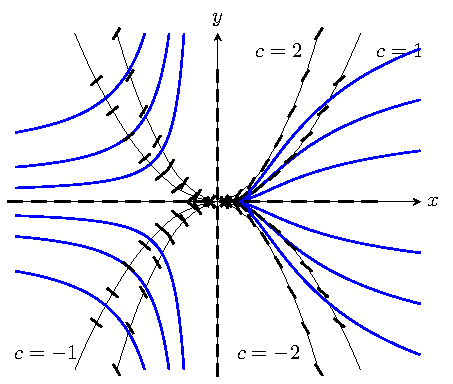
\includegraphics[scale=2]{pr3.pdf}
        % \import{../tikz/}{pr3.tikz}
    \end{figure}
    Finally we draw several smooth curves. These smooth curves complete the phase portrait of \eqref{eq:p2a.1}.
\end{soln}


\begin{soln}[b]
    We have
    \begin{equation}
        \begin{rcases}
            \displaystyle\dot{x}=x(4-2x-4y)\quad\\
            \displaystyle\dot{y}=y(x-1)
        \end{rcases}
        \label{eq:p2b.1}
    \end{equation}
    The critical point of the system \eqref{eq:p2b.1} are given by \(\dot{x}=0\) and \(\dot{y}=0\). i.e.,
    \begin{align}
        x(4-2x-4y)&=0\label{eq:p2b.2}\\
        y(x-1)&=0\label{eq:p2b.3}
    \end{align}
    From \eqref{eq:p2b.3} we get, \(y=0\), \(x=1\)\\
    Putting \(y=0\) in \eqref{eq:p2b.2} we get, \(x=0\), \(x=2\)\\
    Putting \(x=1\) in \eqref{eq:p2b.2} we get, \(y=1/2\)\\


    Hence, the critical points are \((0,0)\), \((2,0)\), \((1,\frac{1}{2})\).\\
    
    
    \emph{(I) Investigation for critical point \((0,0)\):}\\
    The corresponding linearized system of \eqref{eq:p2b.1} is 
    \begin{equation}
        \begin{rcases}
            \dot{x}=4x\\
            \dot{y}=-y\quad
        \end{rcases}
        \label{eq:p2b.4}
    \end{equation}
    Here we observe that
    \begin{enumerate}[label=(\roman*)]
        \item \(\begin{vmatrix}
            a&b\\
            c&d
        \end{vmatrix}=\begin{vmatrix}
            4&0\\
            0&-1
        \end{vmatrix}\neq 0\)
        \item \(\displaystyle\lim_{\substack{x\to 0 \\ y\to 0}} \frac{P(x,y)}{\sqrt{x^2+y^2}}=\lim_{\substack{x\to 0 \\ y\to 0}} \frac{Q(x,y)}{\sqrt{x^2+y^2}}=0\)\\ 
        
        Where \(P(x,y)=-2x^2-4xy\) and \(Q(x,y)=xy\)
    \end{enumerate}
    Hence the behavior of the paths of the system \eqref{eq:p2b.1} near \((0,0)\) would be similar to that of the paths of the related linearized system \eqref{eq:p2b.4}.\\
    The characteristic equation of \eqref{eq:p2b.4} is
    \begin{align*}
        &\lambda^2-(4-1)\lambda-4-0=0\\
        \Rightarrow\;&\lambda^2-3\lambda-4=0\\
        \Rightarrow\;&\lambda^2-4\lambda+\lambda-4=0\\
        \Rightarrow\;&\lambda=4,\;\;-1
    \end{align*}
    The characteristic roots are real, unequal and of opposite sign. Hence, not only \((0,0)\) is an unstable saddle point of the system \eqref{eq:p2b.4} but also an unstable saddle point of the system \eqref{eq:p2b.1}.\\
    
    
    \emph{(II) Investigation for critical point \((2,0)\):}\\
    For the critical point \((2,0)\) we make the transformation \(x=\xi+2\), \(y=\eta\). So that \(\dot{x}=\dot{\xi}\), \(\dot{y}=\dot{\eta}\). Which transforms the critical point \(x=2\), \(y=0\) to \(\xi=0\), \(\eta=0\) in the \(\xi\eta\) plane.\\
    With this transformation, we get from \eqref{eq:p2b.1}
    \begin{align}
        &\dot{\xi}=4(\xi+2)-2(\xi+2)^2-4(\xi+2)\eta\notag\\
        &\dot{\eta}=\eta(\xi+2)-\eta\notag\\
        \Rightarrow\;\;&\begin{aligned}
            \begin{rcases}
                \dot{\xi}=-4\xi-8\eta-2\xi^2-4\xi\eta\quad\\
                \dot{\eta}=\eta+\xi\eta
            \end{rcases}
        \end{aligned}\label{eq:p2b.5}
    \end{align}
    The corresponding linearized system of \eqref{eq:p2a.5} is 
    \begin{equation}
        \begin{rcases}
            \dot{\xi}=-4\xi-8\eta\quad\\
            \dot{\eta}=\eta\quad
        \end{rcases}
        \label{eq:p2b.6}
    \end{equation}
    Here we observe that
    \begin{enumerate}[label=(\roman*)]
        \item \(\begin{vmatrix}
            a&b\\
            c&d
        \end{vmatrix}=\begin{vmatrix}
            -4&-8\\
            0&1
        \end{vmatrix}\neq 0\)
        \item \(\displaystyle\lim_{\substack{\xi\to 0 \\ \eta\to 0}} \frac{P_1(\xi,\eta)}{\sqrt{\xi^2+\eta^2}}=\lim_{\substack{\xi\to 0 \\ \eta\to 0}} \frac{Q_1(\xi,\eta)}{\sqrt{\xi^2+\eta^2}}=0\)\\ 
        
        Where \(P_1(\xi,\eta)=-2\xi^2-4\xi\eta\), and \(Q_1(\xi,\eta)=\xi\eta\)
    \end{enumerate}
    Hence the behavior of the paths of the system \eqref{eq:p2b.5} near \((0,0)\) would be similar to that of the paths of the related linearized system \eqref{eq:p2b.4}.\\
    The characteristic equation of \eqref{eq:p2a.6} is
    \begin{align*}
        &\lambda^2-(-4+1)\lambda-4=0\\
        \Rightarrow\;&\lambda^2+3\lambda-4=0\\
        \Rightarrow\;&\lambda^2+4\lambda-\lambda-4=0\\
        \Rightarrow\;&\lambda=-4,\;\;1
    \end{align*}
    Since the characteristic roots are real, unequal and of opposite sign. Hence, not only \((0,0)\) is an unstable saddle point of the system \eqref{eq:p2b.6} but also an unstable saddle point of the system \eqref{eq:p2b.5}. So the critical
    point \((0,-\frac{1}{3})\) is an unstable saddle point of the system \eqref{eq:p2b.1}.\\
    
    
    \emph{(III) Investigation for critical point \((1,1/2)\):}\\
    For the critical point \((1,1/2)\) we make the transformation \(x=\xi_1+1\), \(y=\eta_1+\frac{1}{2}\). So that \(\dot{x}=\dot{\xi}_1\), \(\dot{y}=\dot{\eta}_1\). Which transforms the critical point \(x=1\), \(y=\frac{1}{2}\) to \(\xi_1=0\), \(\eta_1=0\) in the \(\xi_1\eta_1\) plane.\\
    With this transformation, we get from \eqref{eq:p2b.1}
    \begin{align}
        &\dot{\xi}=4(\xi_1+1)-2(\xi_1+1)^2-4(\xi_1+1)\left(\eta_1+\frac{1}{2}\right)\notag\\
        &\dot{\eta}=\left( \eta_1+\frac{1}{2} \right)(\xi_1+1)-\left( \eta_1+\frac{1}{2} \right)\notag\\
        \Rightarrow\;\;&\begin{aligned}
            \begin{rcases}
                \dot{\xi}=-2\xi_1-4\eta_1-2\xi_1^2-4\xi_1\eta_1\quad\\
                \dot{\eta}=\frac{1}{2}\xi_1+\xi_1\eta_1
            \end{rcases}
        \end{aligned}\label{eq:p2b.7}
    \end{align}
    The corresponding linearized system of \eqref{eq:p2b.7} is 
    \begin{equation}
        \begin{rcases}
            \dot{\xi}_1=2\xi_1-4\eta_1\\
            \dot{\eta}_1=\frac{1}{2}\xi_1\quad
        \end{rcases}
        \label{eq:p2b.8}
    \end{equation}
    Here we observe that
    \begin{enumerate}[label=(\roman*)]
        \item \(\begin{vmatrix}
            a&b\\
            c&d
        \end{vmatrix}=\begin{vmatrix}
            -2&-4\\
            \frac{1}{2}&0
        \end{vmatrix}\neq 0\)
        \item \(\displaystyle\lim_{\substack{\xi_1\to 0 \\ \eta_1\to 0}} \frac{P_2(\xi_1,\eta_1)}{\sqrt{\xi_1^2+\eta_1^2}}=\lim_{\substack{\xi_1\to 0 \\ \eta_1\to 0}} \frac{Q_2(\xi_1,\eta_1)}{\sqrt{\xi_1^2+\eta_1^2}}=0\)\\ 
        
        Where \(P_2(\xi_1,\eta_1)=-2\xi_1^2-4\xi_1\eta_1\) and \(Q_2(\xi_1,\eta_1)=\xi_1\eta_1\)
    \end{enumerate}
    Hence the behavior of the paths of the system \eqref{eq:p2b.7} near \((0,0)\) would be similar to that of the paths of the related linearized system \eqref{eq:p2b.8}.\\
    The characteristic equation of \eqref{eq:p2a.6} is
    \begin{align*}
        &\lambda^2+2\lambda+2=0\\
        \Rightarrow\;&\lambda=\frac{-2\pm \sqrt{4-8}}{2}\\
        \Rightarrow\;&\lambda=-1\pm i
    \end{align*}
    Since the characteristic roots are conjugate complex with negative real parts. Hence, \((0,0)\) is an asymptotically stable spiral point of the system \eqref{eq:p2b.8} and hence of \eqref{eq:p2b.7}. So the critical
    point \((2,1)\) is an asymptotically stable spiral point of \eqref{eq:p2a.1}.\\



    Finally, we get the critical point 
    \begin{enumerate}[label=(\roman*)]
        \item \((0,0)\) is an unstable saddle point of \eqref{eq:p2b.1}
        \item \((2,0)\) is an unstable saddle point of \eqref{eq:p2b.1}
        \item \((1,1/2)\) is an asymptotically stable spiral point of \eqref{eq:p2b.1}
    \end{enumerate}

    \emph{Phase Portrait:} From \eqref{eq:p2b.1} we get
    \[\ddx{y}=\frac{y(x-1)}{x(4-2x-4y)}\]
    The isocline of the above differential equation are given by
    \begin{align*}
        &\ddx{y}=c\\
        \Rightarrow\;&\frac{y(x-1)}{x(4-2x-4y)}=c
    \end{align*}
    Where \(c\) is the slope of the line element of the canvas obtained for different values of \(c\).\\
    When \(c=0\), then \(y=0,\,\,x=1\) and \(\theta=0^{\circ}\)\\
    When \(c=\infty\), then \(x=0\;\;\,2x+4y=4\,\Rightarrow\;\frac{x}{2}+\frac{y}{1}\) and \(\theta=90^{\circ}\)
    \begin{figure}[H]
        \centering
        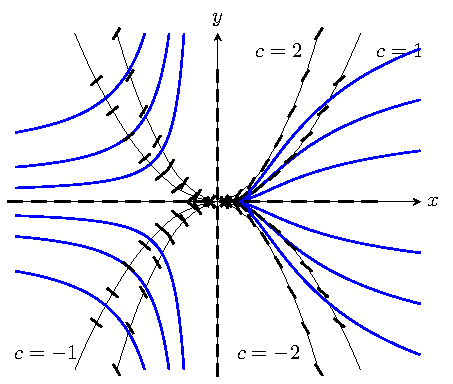
\includegraphics[scale=2]{pr3.pdf}
        % \import{../tikz/}{pr3.tikz}
    \end{figure}
    Finally we draw several smooth curves. These smooth curves complete the phase portrait of \eqref{eq:p2b.1}.
\end{soln}

\begin{soln}[c]
    We have
    \begin{equation}
        \begin{rcases}
            \displaystyle\dot{x}=y-x^2\quad\\
            \displaystyle\dot{y}=8x-y^2
        \end{rcases}
        \label{eq:p2c.1}
    \end{equation}
    The critical point of the system \eqref{eq:p2c.1} are given by \(\dot{x}=0\) and \(\dot{y}=0\). i.e.,
    \begin{align}
        y-x^2&=0\label{eq:p2c.2}\\
        8x-y^2&=0\label{eq:p2c.3}
    \end{align}
    Substituting \eqref{eq:p2c.2} in \eqref{eq:p2c.3} we get
    \begin{align*}
        &8x-x^4=0\\
        \Rightarrow\,&x(8-x^3)=0\\
        \Rightarrow\,&x=0,\;\;x=2
    \end{align*}
    Putting \(x=2\) in \eqref{eq:p2c.2} we get, \(y=0\), \(y=4\)\\


    Hence, the critical points are \((0,0)\), \((2,4)\).\\
    
    
    \emph{(I) Investigation for critical point \((0,0)\):}\\
    The corresponding linearized system of \eqref{eq:p2c.1} is 
    \begin{equation}
        \begin{rcases}
            \dot{x}=y\\
            \dot{y}=8x\quad
        \end{rcases}
        \label{eq:p2c.4}
    \end{equation}
    Here we observe that
    \begin{enumerate}[label=(\roman*)]
        \item \(\begin{vmatrix}
            a&b\\
            c&d
        \end{vmatrix}=\begin{vmatrix}
            0&1\\
            8&0
        \end{vmatrix}\neq 0\)
        \item \(\displaystyle\lim_{\substack{x\to 0 \\ y\to 0}} \frac{P(x,y)}{\sqrt{x^2+y^2}}=\lim_{\substack{x\to 0 \\ y\to 0}} \frac{Q(x,y)}{\sqrt{x^2+y^2}}=0\)\\ 
        
        Where \(P(x,y)=-x^2\) and \(Q(x,y)=-y^2\)
    \end{enumerate}
    Hence the behavior of the paths of the system \eqref{eq:p2c.1} near \((0,0)\) would be similar to that of the paths of the related linearized system \eqref{eq:p2c.4}.\\
    The characteristic equation of \eqref{eq:p2c.4} is
    \begin{align*}
        &\lambda^2-8=0\\
        % \Rightarrow\;&\lambda^2-3\lambda-4=0\\
        % \Rightarrow\;&\lambda^2-4\lambda+\lambda-4=0\\
        \Rightarrow\;&\lambda=\pm 2\sqrt{2}
    \end{align*}
    The characteristic roots are real, unequal and of opposite sign. Hence, not only \((0,0)\) is an unstable saddle point of the system \eqref{eq:p2c.4} but also an unstable saddle point of the system \eqref{eq:p2c.1}.\\
    
    
    \emph{(II) Investigation for critical point \((2,4)\):}\\
    For the critical point \((2,4)\) we make the transformation \(x=\xi+2\), \(y=\eta+4\). So that \(\dot{x}=\dot{\xi}\), \(\dot{y}=\dot{\eta}\). Which transforms the critical point \(x=2\), \(y=4\) to \(\xi=0\), \(\eta=0\) in the \(\xi\eta\) plane.\\
    With this transformation, we get from \eqref{eq:p2c.1}
    \begin{align}
        &\dot{\xi}=4+\eta-(\xi+2)^2\notag\\
        &\dot{\eta}=8(\xi+2)-(\eta+4)^2\notag\\
        \Rightarrow\;\;&\begin{aligned}
            \begin{rcases}
                \dot{\xi}=-4\xi+\eta-\xi^2\quad\\
                \dot{\eta}=8\xi-8\eta-\eta^2
            \end{rcases}
        \end{aligned}\label{eq:p2c.5}
    \end{align}
    The corresponding linearized system of \eqref{eq:p2c.5} is 
    \begin{equation}
        \begin{rcases}
            \dot{\xi}=-4\xi+\eta\quad\\
            \dot{\eta}=8\xi-8\eta\quad
        \end{rcases}
        \label{eq:p2c.6}
    \end{equation}
    Here we observe that
    \begin{enumerate}[label=(\roman*)]
        \item \(\begin{vmatrix}
            a&b\\
            c&d
        \end{vmatrix}=\begin{vmatrix}
            -4&1\\
            8&-8
        \end{vmatrix}\neq 0\)
        \item \(\displaystyle\lim_{\substack{\xi\to 0 \\ \eta\to 0}} \frac{P_1(\xi,\eta)}{\sqrt{\xi^2+\eta^2}}=\lim_{\substack{\xi\to 0 \\ \eta\to 0}} \frac{Q_1(\xi,\eta)}{\sqrt{\xi^2+\eta^2}}=0\)\\ 
        
        Where \(P_1(\xi,\eta)=-\xi^2\), and \(Q_1(\xi,\eta)=-\eta^2\)
    \end{enumerate}
    Hence the behavior of the paths of the system \eqref{eq:p2c.6} near \((0,0)\) would be similar to that of the paths of the related linearized system \eqref{eq:p2c.5}.\\
    The characteristic equation of \eqref{eq:p2c.6} is
    \begin{align*}
        &\lambda^2-(-4-8)\lambda+32-8=0\\
        \Rightarrow\;&\lambda^2+12\lambda+24=0\\
        % \Rightarrow\;&\lambda^2+4\lambda-\lambda-4=0\\
        \Rightarrow\;&\lambda=-6\pm\sqrt{12}
    \end{align*}
    Since the characteristic roots are real, unequal and of negative sign. Hence, not only \((0,0)\) is an asymptotically stable node of the system \eqref{eq:p2c.6} but also an asymptotically stable node of the system \eqref{eq:p2c.5}. So the critical
    point \((2,4)\) is an asymptotically stable node of the system \eqref{eq:p2c.1}.\\


    Finally, we get the critical point 
    \begin{enumerate}[label=(\roman*)]
        \item \((0,0)\) is an unstable saddle point of \eqref{eq:p2b.1}
        % \item \((2,0)\) is an unstable saddle point of \eqref{eq:p2b.1}
        \item \((2,4)\) is an asymptotically stable node of \eqref{eq:p2c.1}
    \end{enumerate}

    \emph{Phase Portrait:} From \eqref{eq:p2c.1} we get
    \[\ddx{y}=\frac{8x-y^2}{y-x^2}\]
    The isocline of the above differential equation are given by
    \begin{align*}
        &\ddx{y}=c\\
        \Rightarrow\;&\frac{8x-y^2}{y-x^2}=c
    \end{align*}
    Where \(c\) is the slope of the line element of the canvas obtained for different values of \(c\).\\
    When \(c=0\), then \(y^2=8x\) and \(\theta=0^{\circ}\)\\
    When \(c=\infty\), then \(y=x^2\) and \(\theta=90^{\circ}\)
    \begin{figure}[H]
        \centering
        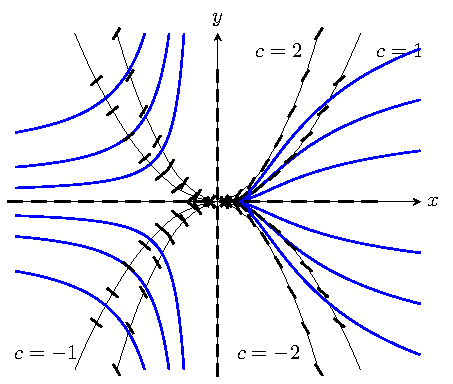
\includegraphics[scale=2]{pr3.pdf}
        % \import{../tikz/}{pr3.tikz}
    \end{figure}
    Finally we draw several smooth curves. These smooth curves complete the phase portrait of \eqref{eq:p2c.1}.
\end{soln}
\end{document}